\section{Concepto de VO}
\begin{frame}
\frametitle{Concepto de VO}
\emph{``En la actualidad se está generando una ingente cantidad de datos
provenientes de un número creciente de instrumentos astronómicos con cada vez
mejor resolución, lo que está multiplicando las neceisdades de almacenamiento''.}
\footnote{El Observatorio virtual, Por Juan de Dios Santander (IAA-CSIC)}


Algunas necesidades:
\newline
\begin{itemize}%[<+->]
	\transdissolve
	\setlength{\itemindent}{1.0cm}
	\item <2->Facilidad de acceso
	\item <3->Información relativa a los datos
	\item <4->Procesamiento de datos
	\item <5->Minería de datos
\end{itemize}

\end{frame}

\subsection{Protocolos y estándares IVOA}
\begin{frame}
\frametitle{Protocolos y estándares IVOA}
\begin{multicols}{2}
La misión de IVOA es facilitar la coordinación y colaboración necesaria para
facilitar el acceso global e integrado a los datos recogidos por los
observatorios astronómicos internacionales.

\textbf{Principal función}: crear, versionar e informar acerca de los
protocolos y estándares. %\cite{ivoa_documents}. 

\textbf{Working Groups}. Preparan documentos para especificar funcionalidades,
arquitecturas, normas, etc. de observatorio virtual.

Este proceso se realiza de la siguiente forma~\ref{fig:creacionestandares}.
\begin{figure}[h!t]
        \centering
         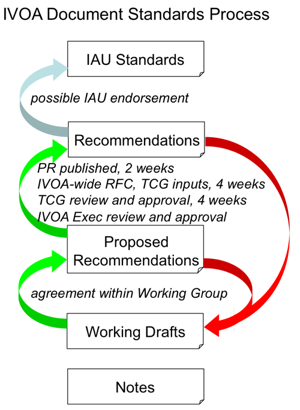
\includegraphics[width=0.45\textwidth]{img/diagrama_proceso.png}
         %\caption{Creación de Estándares IVOA}
        \label{fig:creacionestandares}
\end{figure}
\end{multicols}
\end{frame}

\subsection{Working Groups}
\begin{frame}
\frametitle{Working Groups}
\begin{multicols}{2}
Los principales Working Groups estan relacionados a:
\begin{itemize}
	\item <2-> \textbf{Aplicaciones}: herramientas de software de astronomía.
	\item <3-> \textbf{Capa acceso a los datos}: acceso remoto a los datos.
	\item <4-> \textbf{Modelamiento de datos}: descripción de los metadatos de una observación.
	\item <5-> \textbf{Grid y servicios web}: tecnologías de redes e internet.
	\item <6-> \textbf{Registro de recursos}: registro, localización y uso de recursos de VO.
	\item <7-> \textbf{Semánticas}: significado o interpretaciones o tipos de lenguajes en el contexto.
	\item <8-> \textbf{Eventos VO}: información acerca eventos celestiales transitorios.
\end{itemize}

\end{multicols}
\end{frame}
